\begin{frame}{Contracting boattails improve across three RASAero rocket families}
\centering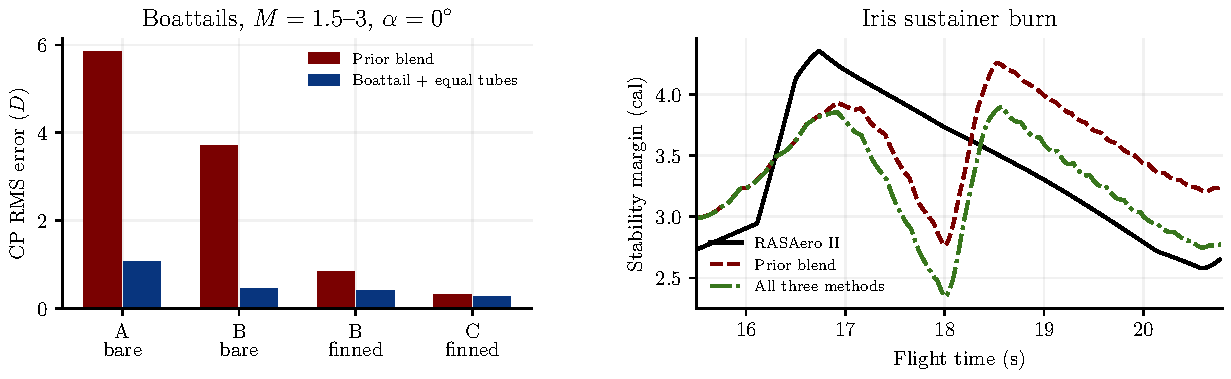
\includegraphics[width=.96\linewidth,height=.58\textheight,keepaspectratio]{figures/afterbody-comparison.pdf}
\begin{columns}[T,onlytextwidth]
\column{.48\textwidth}\small\textbf{Boattails.} The reserved four-fin rocket improved at every tested incidence. At $2^\circ$, RMS error in the moment added by its taper fell from 0.076 to 0.008. ARCAS tunnel CP error rose from 0.31 to $0.36D$.
\column{.48\textwidth}\small\textbf{Iris.} The stepped-center model brought burnout from 3.24 to 2.77 cal. RASAero gave 2.65. The modeled minimum fell to 2.35 cal at 18.00 s. RASAero gave 2.58 cal at 20.60 s.
\end{columns}
\end{frame}
\begin{frame}{Which components merit a change in MIT 6.6?}
\begin{columns}[T,onlytextwidth]
\column{.48\textwidth}
\begin{block}{Join identical tubes}
Drawing the same 48-inch cylinder as four tubes moved CP by up to $0.70D$ in the prior blend. Using its continuous length eliminated the difference at all 453 tested conditions.
\end{block}
\begin{block}{Evaluate contracting boattails}
Use the DATCOM normal-force increment and its own local load station. Agreement with native RASAero improved on both bare bodies and both finned boattails.
\end{block}
\column{.48\textwidth}
\begin{block}{Keep the other changes experimental}
The stepped-center model increased finless Iris CP error from 2.86 to $4.16D$ at zero incidence. The tested flare correction worsened the measured flare-minus-cylinder moment. The crossflow change gave mixed finite-incidence results.
\end{block}
\small\textbf{Verification.} Thirteen fresh native static models, three archived Iris geometries, two native field diagnostics, three tunnel datasets and a full two-stage Iris rerun in the Windows VM.
\end{columns}
\end{frame}
